\documentclass[a4paper,fleqn]{cas-sc}
\usepackage[authoryear]{natbib}
\usepackage[T1]{fontenc}
\usepackage[utf8]{inputenc}
\usepackage{lineno}
\usepackage{booktabs}
\usepackage{url}
\linenumbers

\begin{document}
\let\WriteBookmarks\relax
\def\floatpagepagefraction{1}
\def\textpagefraction{.001}

\shorttitle{Fotossíntese líquida MODIS ao longo de um gradiente hidroclimático tropical}
\shortauthors{Y.A.S. Oliveira et al.}

\title[mode = title]{Regressão polinomial regularizada da fotossíntese líquida MODIS ao longo de um gradiente hidroclimático tropical: Mata Atlântica, Cerrado e Caatinga no Nordeste do Brasil (2001--2025)}

\author[1]{Ygor Augusto dos Santos Oliveira}[orcid=0009-0001-5821-658X]
\cormark[1]
\ead{ygornayty2@gmail.com}
\credit{Conceituação, Metodologia, Software, Análise formal, Curadoria de dados, Redação -- rascunho original}

\author[1]{Nayanne Silva Benfica}
\credit{Conceituação, Metodologia, Curadoria de dados, Redação -- revisão e edição, Supervisão}

\author[1]{Fabrício Berton Zanchi}[orcid=0000-0002-8074-2893]
\credit{Conceituação, Metodologia, Redação -- revisão e edição, Supervisão}

\affiliation[1]{organization={Programa de Pós-graduação em Ciências e Tecnologias Ambientais, Universidade Federal do Sul da Bahia / Instituto Federal de Educação, Ciência e Tecnologia da Bahia},
  city={Porto Seguro},
  postcode={45810-000},
  state={Bahia},
  country={Brasil}}

\cortext[1]{Autor para correspondência}

\begin{abstract}
Os biomas Mata Atlântica, Cerrado e Caatinga do Estado da Bahia respondem de forma distinta ao clima, e essas respostas raramente são lineares. Este estudo desenvolveu e validou um modelo de regressão múltipla polinomial, estimado por regressão Ridge, para a Fotossíntese Líquida (PSN) mensal dos três biomas entre 2001 e 2025, a partir de produtos MODIS e da precipitação GPM IMERG. Os preditores candidatos foram evapotranspiração, precipitação, temperatura da superfície, índice de disponibilidade hídrica e área queimada, além de duas componentes harmônicas do ciclo anual. O grau polinomial e o conjunto de preditores foram selecionados por validação cruzada repetida, e a seleção e o desempenho foram verificados por validação agrupada por ano, por blocos cronológicos e por nulos que preservam a estrutura temporal da série. O modelo de grau 2 explicou 96,7\% da variância da PSN no Cerrado, 94,2\% na Caatinga e 73,7\% na Mata Atlântica, com queda máxima de 6,7 pontos sob validação cronológica. No Cerrado, o índice de disponibilidade hídrica foi selecionado em lugar da temperatura na combinação de melhor desempenho, com diferença pequena mas consistente entre partições; na Mata Atlântica, contribuiu apenas por interação com a evapotranspiração e a temperatura. A remoção das componentes harmônicas reduziu o desempenho em 21,8 pontos na Mata Atlântica e em menos de 3 pontos nos biomas sazonais, e mostrou que a contribuição aparente da precipitação decorre em grande parte do ciclo anual. Os resultados caracterizam três padrões distintos de associação entre clima e produtividade e indicam que a regressão polinomial regularizada é uma alternativa reprodutível e interpretável para o monitoramento da vegetação por sensoriamento remoto.
\end{abstract}

\begin{highlights}
\item Polinômio de grau 2 com Ridge explicou 97\%, 94\% e 74\% da PSN mensal em três biomas
\item Grau, conjunto de variáveis e desempenho mantidos sob validação por anos e cronológica
\item No Cerrado, o índice de disponibilidade hídrica foi selecionado em lugar da temperatura
\item Com sazonalidade explícita, a contribuição dos preditores reflete anomalias, não o calendário
\item Três padrões de associação: limitação hídrica, resposta pulsada e resposta multifatorial
\end{highlights}

\begin{keywords}
MODIS \sep Fotossíntese líquida \sep Regressão Ridge \sep Sazonalidade \sep Biomas brasileiros \sep Validação temporal
\end{keywords}

\maketitle

\section{Introdução}\label{sec:intro}

A Fotossíntese Líquida (PSN) é o carbono assimilado pela vegetação após o desconto da respiração de manutenção de folhas e raízes finas e, por isso, responde de forma quase imediata às condições ambientais \citep{running2004,running2021gpp}. Em escala mensal, a PSN é um indicador mais direto da atividade fotossintética do que a produtividade primária líquida integrada anualmente e tem sido utilizada para acompanhar a resposta da vegetação a fatores climáticos e antrópicos \citep{nemani2003,benfica2023}. Os biomas Mata Atlântica, Cerrado e Caatinga do Estado da Bahia são áreas prioritárias para a conservação submetidas a pressões distintas: fragmentação florestal e silvicultura na faixa litorânea, expansão da fronteira agrícola no oeste do Cerrado e degradação e desertificação no semiárido \citep{ribeiro2009,lima2020,marengo2018,mapbiomas2025}. Para esses biomas, \citet{benfica2022,benfica2023} mostraram que a PSN se correlaciona positivamente com a evapotranspiração e com um índice de disponibilidade hídrica e negativamente com a temperatura da superfície, com maior sensibilidade climática no Cerrado e na Caatinga.

Essas relações, contudo, raramente são lineares. A produtividade aumenta com a disponibilidade de água apenas até determinado ponto, a partir do qual satura ou declina, e estudos empíricos documentam limiares de precipitação abaixo dos quais a produtividade responde de forma mais intensa \citep{jin2018,linger2020,mwangi2025}. Em escala mais ampla, a ecologia teórica descreve os ecossistemas como sistemas complexos, com transições críticas e dependência de contexto \citep{levin1998,flores2024}, e as avaliações do IPCC ressaltam que as respostas a pressões combinadas envolvem limiares e interações \citep{ipcc2022}. Entre as alternativas não lineares, os métodos de aprendizado de máquina têm dominado a estimativa de produtividade por sensoriamento remoto, com bom desempenho preditivo mas pouca transparência sobre a forma das relações ajustadas. A regressão múltipla com termos polinomiais e de interação ocupa uma posição intermediária: acomoda curvaturas e efeitos combinados entre preditores e mantém coeficientes interpretáveis. Sua limitação clássica, a multicolinearidade gerada pela própria expansão polinomial, é contornada pela regressão Ridge, que penaliza a magnitude dos coeficientes e estabiliza a estimação \citep{hoerl1970}. Protocolos de regressão polinomial com seleção combinatória de termos e teste de Y-randomization estão consolidados na modelagem quantitativa estrutura--atividade em química medicinal \citep{guimaraes2024}, mas sua aplicação a séries mensais de produtividade vegetal, com a validação temporal que essas séries exigem, ainda não foi explorada.

Este estudo teve como objetivos (1) desenvolver e validar um Modelo de Regressão Múltipla Polinomial de ordem N (MRMP-N), estimado por regressão Ridge, para a PSN mensal dos biomas Mata Atlântica, Cerrado e Caatinga da Bahia entre 2001 e 2025; (2) determinar empiricamente o grau polinomial e o conjunto de variáveis ambientais de melhor capacidade de generalização em cada bioma, sob esquemas de validação que respeitam a ordem cronológica dos dados; e (3) comparar as associações climáticas da PSN entre os biomas, avaliando como a representação explícita do ciclo anual altera a interpretação da contribuição dos preditores.

\section{Material e métodos}\label{sec:methods}

\subsection{Área de estudo}

Os biomas Mata Atlântica, Cerrado e Caatinga estão localizados no Estado da Bahia, Nordeste do Brasil, e ocupam cerca de 19\%, 27\% e 54\%, respectivamente, dos 564.764~km$^2$ do território estadual \citep{ibge2004,ibge2025} (Fig.~\ref{fig:map}). Segundo a classificação de Köppen para o Brasil \citep{alvares2013}, o litoral e o leste do estado, sob domínio da Mata Atlântica, apresentam clima tropical úmido; o interior e o norte, sob domínio da Caatinga, clima semiárido com precipitação anual entre cerca de 240 e 1.500~mm; e o oeste e o sul, sob domínio do Cerrado, clima tropical com estação seca bem definida. Na Mata Atlântica predominam mosaicos de remanescentes florestais intercalados por pastagens, cacauicultura, silvicultura de eucalipto e áreas urbanas; no oeste do estado, a fronteira agrícola do MATOPIBA converteu extensas áreas de Cerrado em lavouras e pastagens; e na Caatinga a pecuária extensiva, a agricultura de sequeiro e a extração de lenha respondem pela maior parte da conversão da vegetação nativa \citep{mapbiomas2025}.

\begin{figure}
  \centering
  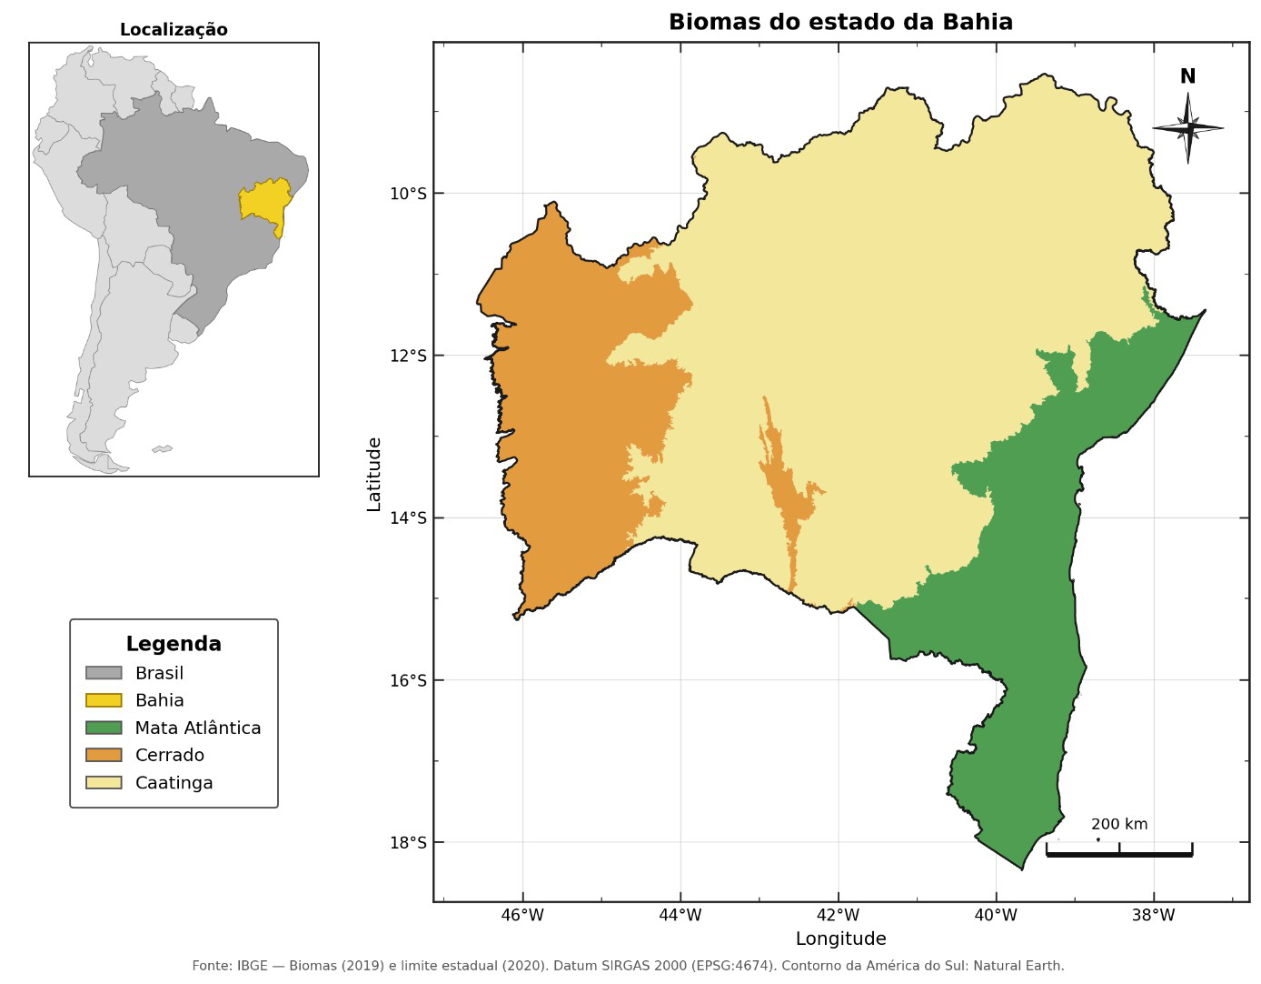
\includegraphics[width=0.8\textwidth]{figs/fig1_map.png}
  \caption{Localização e distribuição dos biomas Mata Atlântica, Cerrado e Caatinga no Estado da Bahia, Brasil \citep[limites de][]{ibge2019}.}\label{fig:map}
\end{figure}

\subsection{Fotossíntese líquida, variáveis climáticas e área queimada}

A PSN foi obtida do produto MOD17A2HGF e a evapotranspiração real (EV) e a potencial (ETP) do produto MOD16A2GF, ambos da Coleção 6.1 do sensor MODIS/Terra, em compostos de oito dias com resolução espacial de 500~m e nas versões com preenchimento de falhas \citep{running2021gpp,running2021et}. A temperatura da superfície terrestre (TST) foi obtida da banda diurna do produto MOD11A2, com resolução de 1~km \citep{wan2021}, e a área queimada (BURN) do produto mensal MCD64A1 \citep{giglio2018}. A precipitação (PRE) foi obtida do produto mensal GPM IMERG Final Run, versão 07, com resolução de 0,1$^\circ$ \citep{huffman2023}, que substituiu a versão 06 utilizada por \citet{benfica2023}. Todos os produtos foram obtidos e processados na plataforma Google Earth Engine \citep{gorelick2017}.

Para cada composto calculou-se a média espacial dos pixels válidos de cada bioma, delimitado pelo mapa de biomas do IBGE na escala 1:250.000 \citep{ibge2019} recortado pelo limite estadual, com os fatores de escala oficiais de cada produto. Consideraram-se válidos os pixels dentro da faixa de valores válidos de cada produto. Para os produtos com preenchimento de falhas (MOD17A2HGF e MOD16A2GF) não se aplicou filtro adicional pela banda de controle de qualidade, uma vez que essas versões já substituem as observações de baixa qualidade por valores interpolados \citep{running2021gpp}, o que não elimina a incerteza inerente a esses produtos. O MOD11A2 não possui versão com preenchimento de falhas: os pixels sem observação de céu claro não recebem valor de TST e ficam fora da média do composto, mas a banda de qualidade QC\_Day, que classifica a incerteza dos pixels retidos, não foi usada como filtro, e a sensibilidade da série de TST a esse filtro não foi avaliada (ver limitações na Discussão). Os compostos foram agregados em janelas fixas de quatro compostos consecutivos, de cerca de 32 dias, reproduzindo a agregação de \citet{benfica2022,benfica2023}: a PSN, a EV e a ETP foram somadas e a TST foi mediada em cada janela. Cada janela foi atribuída ao mês civil que contém a maior parte dos seus dias (janeiro, por exemplo, reúne os compostos iniciados em 27 de dezembro e em 1, 9 e 17 de janeiro), e é a esse mês de referência que se associam as componentes de sazonalidade; os períodos aqui chamados mensais são, portanto, janelas fixas de 32 dias, e não meses civis estritos, o que mantém a comparabilidade com a série original. O índice de disponibilidade hídrica (WAI) foi calculado como a razão EV/ETP e a área queimada como o número de pixels queimados no mês multiplicado pela área do pixel. A série cobre janeiro de 2001 a setembro de 2025 ($n = 297$ meses por bioma); os três últimos meses de 2025 foram excluídos porque a NASA encerrou a versão 07 do IMERG em setembro de 2025 \citep{nasa2026}. A reprodução da base de \citet{benfica2023} por esse procedimento apresentou correlação superior a 0,97 com a série original para todas as variáveis, e a soma anual da PSN correlacionou-se em 0,99 a 1,00 com a NPP anual do produto independente MOD17A3HGF. As variáveis estão descritas na Tabela~\ref{tbl:vars}.

\begin{table}[htbp]
\caption{Variável resposta e preditores candidatos do MRMP-N.}\label{tbl:vars}
\begin{tabular*}{\tblwidth}{@{}LLLL@{}}
\toprule
Variável & Descrição & Unidade & Fonte \\
\midrule
PSN & Fotossíntese líquida (resposta) & gC\,m$^{-2}$\,mês$^{-1}$ & MOD17A2HGF \\
EV & Evapotranspiração real & mm\,mês$^{-1}$ & MOD16A2GF \\
PRE & Precipitação acumulada & mm\,mês$^{-1}$ & GPM IMERG V07 \\
TST & Temperatura da superfície terrestre (diurna) & $^\circ$C & MOD11A2 \\
WAI & Índice de disponibilidade hídrica (EV/ETP) & adimensional & MOD16A2GF \\
BURN & Área queimada, transformada em $\log(1+x)$ & ha & MCD64A1 \\
SAZsin, SAZcos & Componentes harmônicas do ciclo anual & adimensional & Derivadas do mês \\
\bottomrule
\end{tabular*}
\end{table}

\subsection{Modelo de regressão múltipla polinomial}

O MRMP-N segue a arquitetura de regressão polinomial de \citet{guimaraes2024}, adaptada ao contexto ambiental por três decisões: estimação por regressão Ridge com regularização L2 em substituição aos mínimos quadrados ordinários; determinação empírica do grau polinomial entre 1 e 5; e ampliação do protocolo de validação com esquemas temporais. A forma geral do modelo é dada pela Eq.~(\ref{eq:model}), em que $\hat{Y}$ é a PSN estimada, $X_i$ são os preditores padronizados, $\beta_i$ são os coeficientes lineares e $\beta_{ij}$ e $\beta_{ijk}$ os coeficientes dos termos quadráticos e de interação. Os coeficientes são estimados minimizando a função de perda penalizada da Eq.~(\ref{eq:loss}), em que $\alpha$ controla a penalização L2.
\noindent\begin{minipage}{\columnwidth}
\begin{align}
\hat{Y} &= \beta_0 + \sum_i \beta_i X_i + \sum_{i \le j} \beta_{ij} X_i X_j \nonumber\\
        &\quad + \sum_{i \le j \le k} \beta_{ijk} X_i X_j X_k + \dots \label{eq:model}\\
L(\beta) &= \sum_{n=1}^{N} \left(Y_n - \hat{Y}_n\right)^2 + \alpha \sum_{p=1}^{P} \beta_p^2 \label{eq:loss}
\end{align}
\end{minipage}
\vspace{0.5\baselineskip}

Os preditores compreendem três variáveis ambientais, selecionadas entre EV, PRE, TST, WAI e BURN, e duas componentes harmônicas do ciclo anual, $\mathrm{SAZsin} = \operatorname{sen}(2\pi\,\mathrm{mês}/12)$ e $\mathrm{SAZcos} = \cos(2\pi\,\mathrm{mês}/12)$, mantidas fixas em todos os modelos. Como $\beta_1\,\mathrm{SAZsin} + \beta_2\,\mathrm{SAZcos}$ equivale a $A\operatorname{sen}(2\pi\,\mathrm{mês}/12 + \varphi)$, o modelo ajusta livremente a amplitude e a fase do ciclo anual sem impor relações artificiais entre os meses. Para cinco preditores e grau 2, a expansão gera 20 termos (5 lineares, 5 quadráticos e 10 interações entre pares); para um grau N genérico, o número de termos é $\binom{5+N}{N} - 1$, isto é, 55, 125 e 251 termos nos graus 3 a 5. Antes da modelagem, a área queimada foi transformada em $\log(1+x)$, a ETP foi excluída como preditor por sua correlação de 0,73 a 0,80 com a TST, e a PSN do conjunto de treino foi winsorizada no percentil 3 para reduzir a influência de meses de produtividade anormalmente baixa, mantendo-se os valores de teste na escala original; a sensibilidade a essa escolha foi verificada reajustando o modelo com winsorização em 0\%, 1\%, 3\% e 5\%. Todos os preditores foram padronizados por escore-z ajustado exclusivamente sobre o conjunto de treino de cada partição, e $\alpha$ foi selecionado por busca em grade entre 0,1; 1; 10; 50 e 100, com validação cruzada interna de cinco partições, em procedimento aninhado (Fig.~\ref{fig:flow}).

\begin{figure}
  \centering
  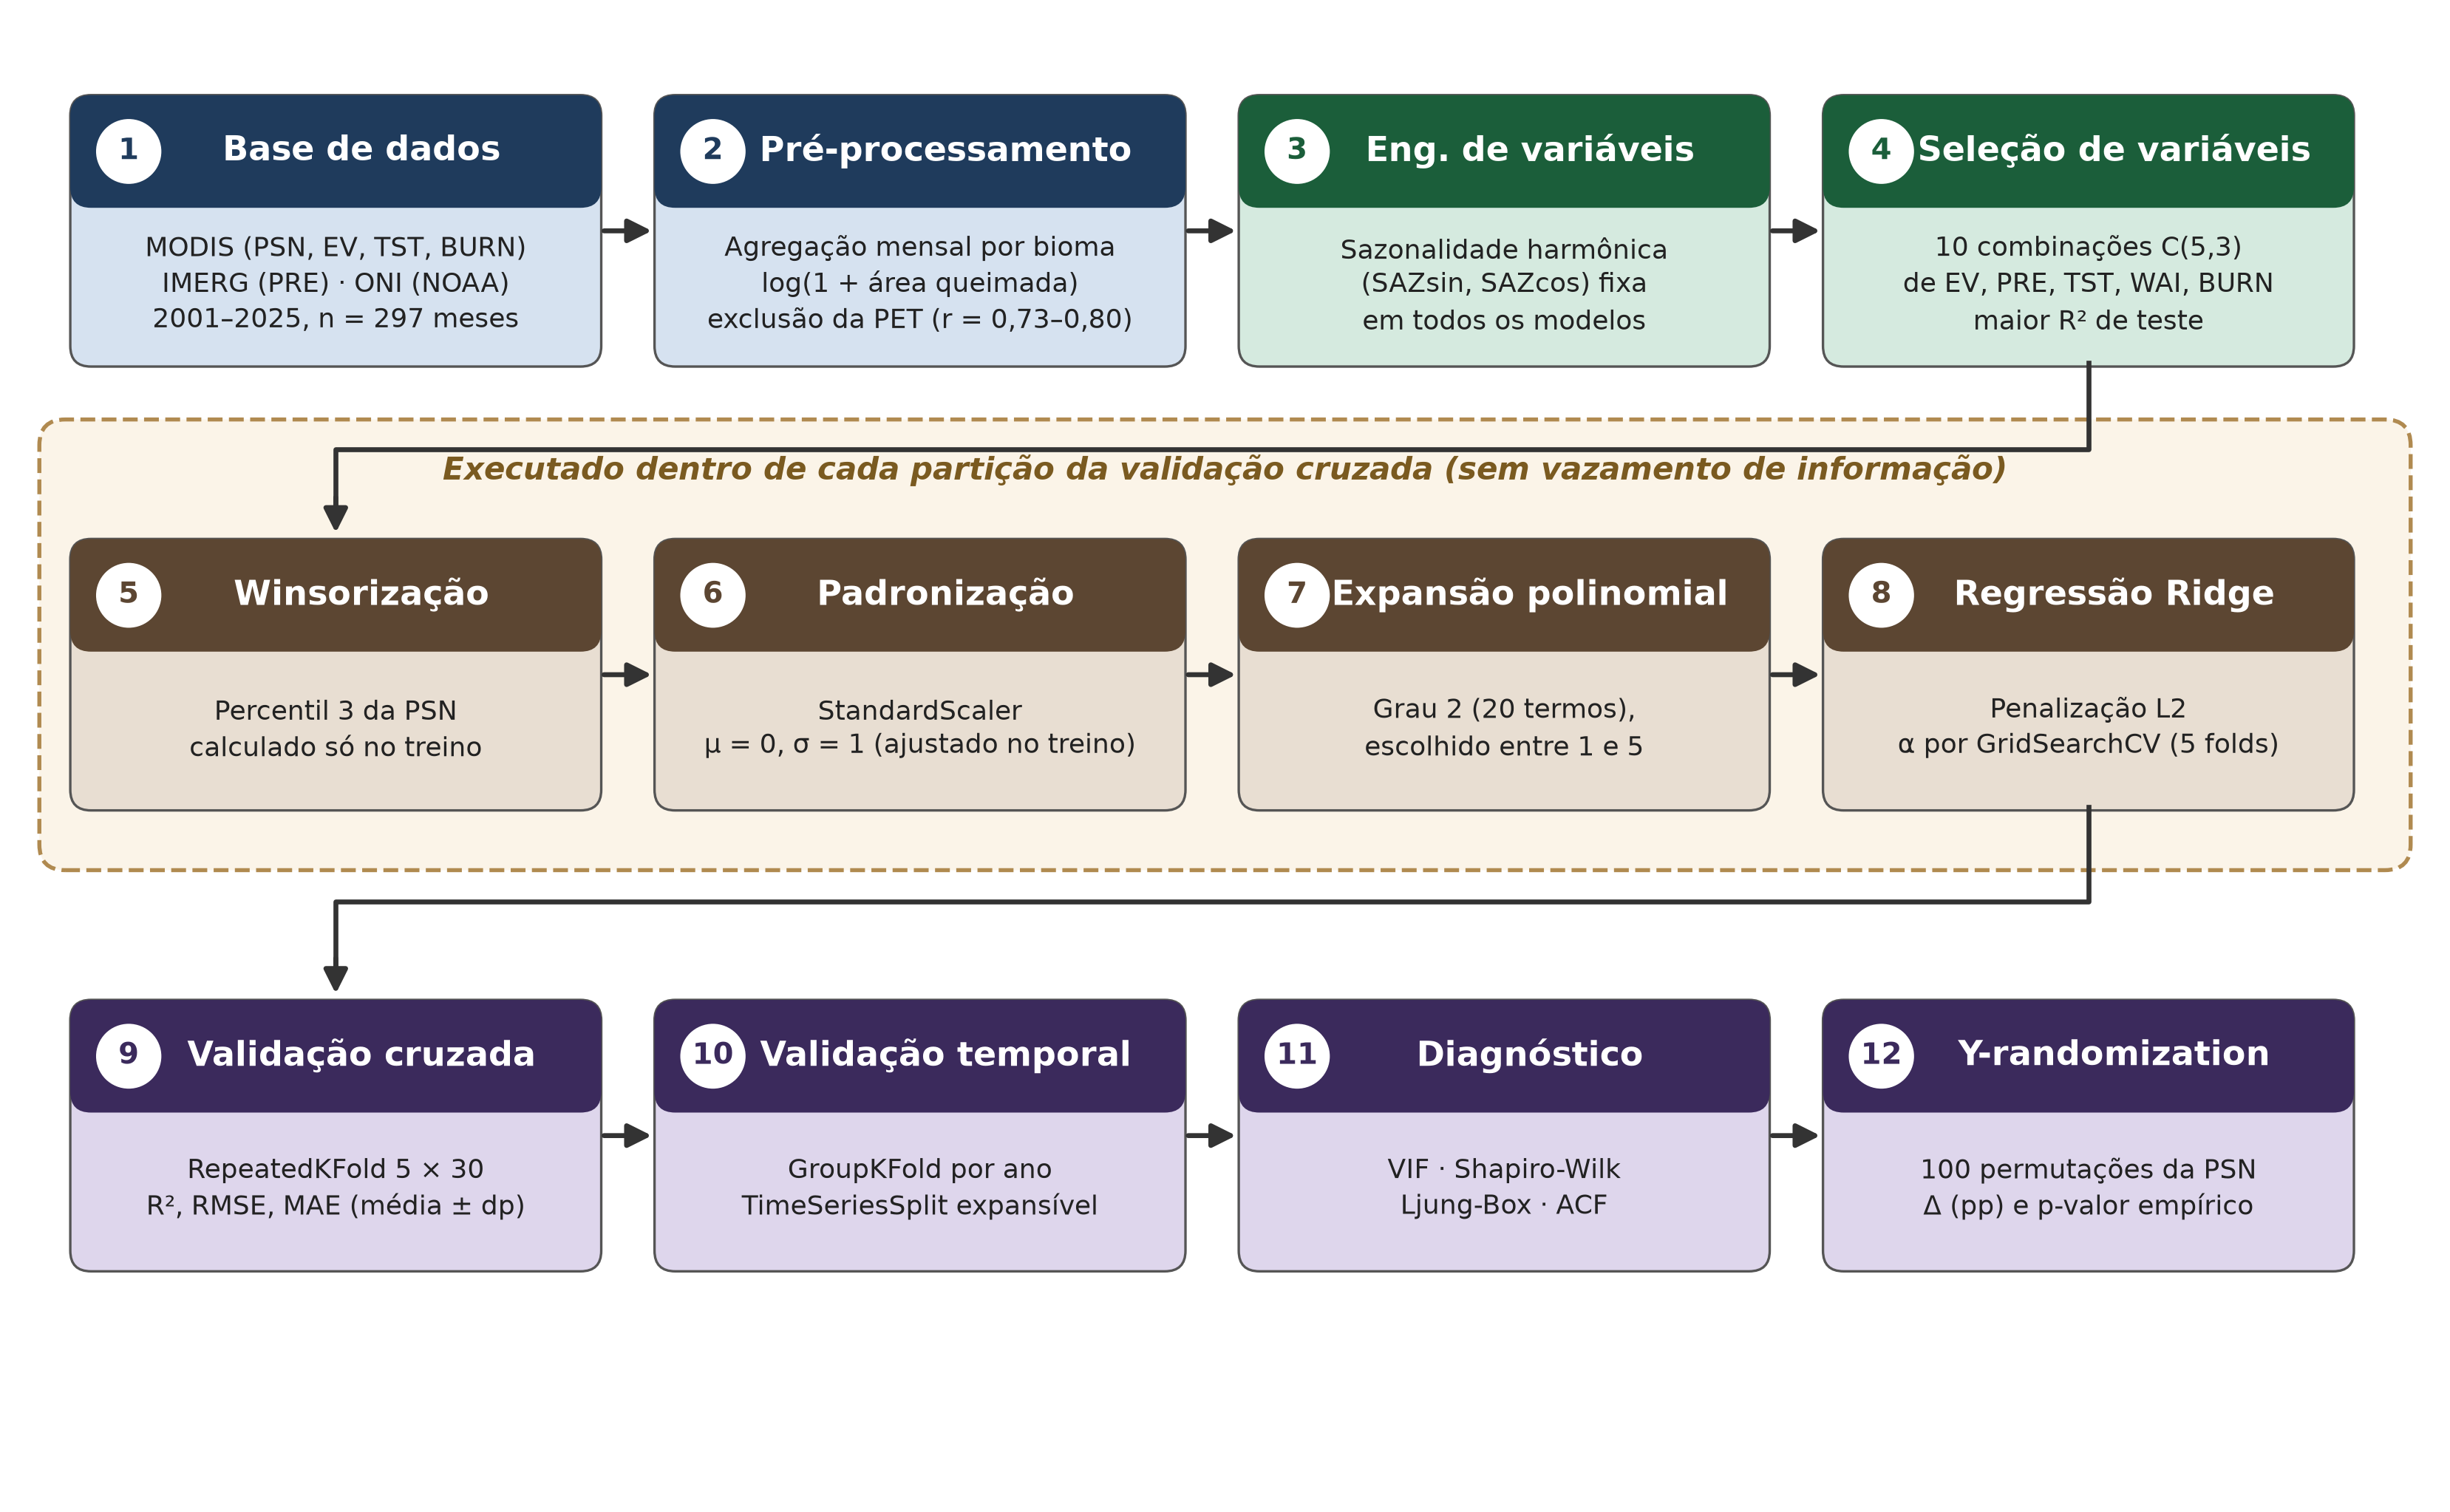
\includegraphics[width=\textwidth]{figs/fig2_workflow.png}
  \caption{Fluxo metodológico do MRMP-N. As etapas 5 a 8 são executadas dentro de cada partição da validação cruzada, sem vazamento de informação entre treino e teste.}\label{fig:flow}
\end{figure}

\subsection{Seleção, validação e análise estatística}

O grau polinomial e o conjunto de preditores foram tratados como hiperparâmetros. Os graus 1 a 5 e as $\binom{5}{3} = 10$ combinações de três variáveis ambientais foram comparados, por bioma, pelo critério composto de maior $R^2$ médio no conjunto de teste e menor diferença entre o $R^2$ de treino e o de teste, adotando-se 10 pontos percentuais como referência orientadora de sobreajuste. A estimativa principal do desempenho veio da validação cruzada RepeatedKFold com cinco partições e trinta repetições (150 partições), reportando-se a média e o desvio-padrão do $R^2$, do RMSE e do MAE de teste e o intervalo empírico de 95\% do $R^2$, definido pelos percentis 2,5 e 97,5 das partições. Como meses vizinhos compartilham estrutura sazonal, o desempenho foi verificado adicionalmente por dois esquemas: o GroupKFold por ano, que mantém anos inteiros fora do treino em cinco blocos de cinco anos, e o TimeSeriesSplit com janela expansível, que ajusta o modelo no passado e o avalia nos 49 meses seguintes, em cinco blocos sucessivos. Apenas o segundo preserva estritamente a ordem cronológica; o primeiro avalia a generalização para anos não utilizados no ajuste e impede que meses consecutivos e autocorrelacionados de um mesmo ano sejam repartidos entre treino e teste.

O índice de contribuição relativa de cada variável foi calculado como a soma dos valores absolutos dos coeficientes padronizados de todos os termos que envolvem a variável, normalizada para 100\% por bioma; trata-se de um índice descritivo do modelo ajustado, e não de uma medida causal. Para avaliar o papel das componentes harmônicas, o modelo final de cada bioma foi reajustado sem elas, sob o mesmo protocolo, e a proporção da variância de cada preditor explicada pelo ciclo anual foi estimada por regressão contra SAZsin e SAZcos. A multicolinearidade foi diagnosticada pelo Fator de Inflação da Variância (VIF) sobre os preditores originais, com os limiares usuais de 5 e 10 tomados como regras práticas e não como critérios absolutos \citep{obrien2007}. A normalidade dos resíduos de um ajuste à série completa foi avaliada pelo teste de Shapiro--Wilk e a autocorrelação pelo teste de Ljung--Box com 12 defasagens. O teste de Y-randomization, adaptado de \citet{guimaraes2024}, reajustou o modelo 100 vezes com a PSN permutada e comparou o $R^2$ de validação cruzada original com o dos modelos permutados por dois indicadores: a distância entre o $R^2$ original e a média dos modelos permutados, reportada de forma descritiva, e um p-valor empírico unilateral, definido como a proporção de permutações cujo $R^2$ iguala ou supera o do modelo original, com significância para $p < 0,05$. Como o grau e o conjunto de variáveis foram escolhidos com base no RepeatedKFold, verificou-se se as mesmas escolhas seriam feitas quando a própria seleção emprega os esquemas temporais: os graus 1 a 5 e as 10 combinações foram reavaliados, com o mesmo pipeline, sob GroupKFold por ano e sob TimeSeriesSplit, registrando-se o grau de maior $R^2$ de teste e a posição da combinação selecionada em cada esquema. A estabilidade da seleção foi ainda medida partição a partição no RepeatedKFold: a frequência com que cada combinação foi a melhor entre as 150 partições e a diferença pareada de $R^2$ de teste entre a primeira e a segunda combinações de cada bioma, com intervalo de confiança de 95\% por bootstrap das partições (5.000 reamostragens) e teste de Wilcoxon pareado.

Como complemento ao índice baseado nos coeficientes, cuja comparabilidade entre termos de ordens diferentes é limitada, calculou-se a importância por permutação \citep{breiman2001} de forma compatível com a dependência temporal: em cada bloco de teste do GroupKFold por ano e do TimeSeriesSplit, o modelo ajustado no treino foi avaliado no teste com cada preditor original embaralhado 20 vezes, antes da expansão polinomial, de modo que todos os termos derivados da variável são afetados em conjunto. A queda média do $R^2$ de teste e a razão entre o RMSE com e sem embaralhamento medem quanto o desempenho fora da amostra depende de cada variável; reportam-se a média e o desvio-padrão entre blocos e a parcela de cada variável na queda total. Como o embaralhamento de um preditor rompe também suas correlações com os demais, variáveis colineares partilham importância, e a medida deve ser lida como preditiva, não causal.

A permutação completa da PSN no Y-randomization destrói toda a dependência temporal da resposta, o que torna o teste pouco exigente em séries autocorrelacionadas. Por isso, o mesmo procedimento ($R^2$ de validação cruzada RepeatedKFold com $\alpha$ fixo) foi repetido sob dois nulos que mantêm a autocorrelação e o ciclo sazonal da PSN: o deslocamento circular da série da PSN em relação aos preditores, para todos os 296 deslocamentos possíveis, entre os quais os 24 múltiplos de 12 meses preservam integralmente o calendário; e a permutação de anos inteiros (100 permutações dos 24 anos completos, mantidos no lugar os nove meses de 2025). Nesses nulos o modelo continua a dispor da sazonalidade e da memória temporal da série; o que se perde é o alinhamento entre a PSN e as condições climáticas do mesmo período. O p-valor empírico foi definido como (número de nulos com $R^2$ igual ou superior ao original + 1)/($n$ + 1). As análises foram realizadas em Python 3.11 com scikit-learn, statsmodels e scipy, com semente aleatória fixa; uma única execução do script do modelo reproduz o ajuste e todas as validações.

\section{Resultados}\label{sec:results}

\subsection{Desempenho preditivo e grau polinomial}

As relações univariadas entre a PSN e os preditores diferiram entre os biomas. No Cerrado e na Caatinga, a evapotranspiração (74,8\% e 76,2\% da variância da PSN) e o WAI (74,1\% e 81,5\%) foram os preditores isolados mais fortes, seguidos da temperatura, com relação negativa (59,2\% e 54,2\%); a precipitação do próprio mês explicou menos de 10\%. Na Mata Atlântica, nenhuma variável isolada explicou mais de 12,5\% da variância da PSN.

O MRMP-N de grau 2 atingiu $R^2$ de teste de 96,7\% no Cerrado, 94,2\% na Caatinga e 73,7\% na Mata Atlântica, com RMSE entre 6,69 e 7,97~gC\,m$^{-2}$\,mês$^{-1}$ e diferença treino--teste de 0,59, 1,03 e 5,19 pontos percentuais (Tabela~\ref{tbl:perf}). A Fig.~\ref{fig:obspred} mostra a correspondência entre a PSN observada e a predita fora da amostra. Sob validação agrupada por ano, o $R^2$ permaneceu praticamente igual ao da validação principal nos três biomas; sob TimeSeriesSplit, manteve-se acima de 91\% no Cerrado e na Caatinga e caiu para 66,98\% na Mata Atlântica, com queda máxima de 6,66 pontos (Tabela~\ref{tbl:perf}). A winsorização em 0\%, 1\%, 3\% ou 5\% alterou o $R^2$ de teste em no máximo 1,3 ponto em qualquer bioma.

\begin{table}[htbp]
\caption{Desempenho preditivo do MRMP-N de grau 2 por bioma: $R^2$ de teste médio ($\pm$ desvio-padrão) com intervalo empírico de 95\%, RMSE e MAE (gC\,m$^{-2}$\,mês$^{-1}$) e diferença treino--teste na validação RepeatedKFold $5 \times 30$, e $R^2$ de teste sob os esquemas de validação temporal. Todos os conjuntos incluem SAZsin e SAZcos.}\label{tbl:perf}
\footnotesize
\begin{tabular*}{\tblwidth}{@{}LLCCCCCCC@{}}
\toprule
Bioma & Conjunto selecionado & $R^2$ teste (\%) & Int.\ emp.\ 95\% (\%) & RMSE & MAE & Dif.\ (pp) & Por ano (\%) & Cronológico (\%) \\
\midrule
Mata Atlântica & EV + TST + WAI & 73,7 $\pm$ 5,9 & 60,1--83,4 & 7,97 & 6,29 & 5,19 & 73,73 & 66,98 \\
Cerrado & EV + PRE + WAI & 96,7 $\pm$ 0,6 & 95,4--97,7 & 6,74 & 5,43 & 0,59 & 96,38 & 95,73 \\
Caatinga & EV + PRE + TST & 94,2 $\pm$ 1,5 & 90,8--96,2 & 6,69 & 5,08 & 1,03 & 93,81 & 91,20 \\
\bottomrule
\end{tabular*}
\end{table}

\begin{figure}
  \centering
  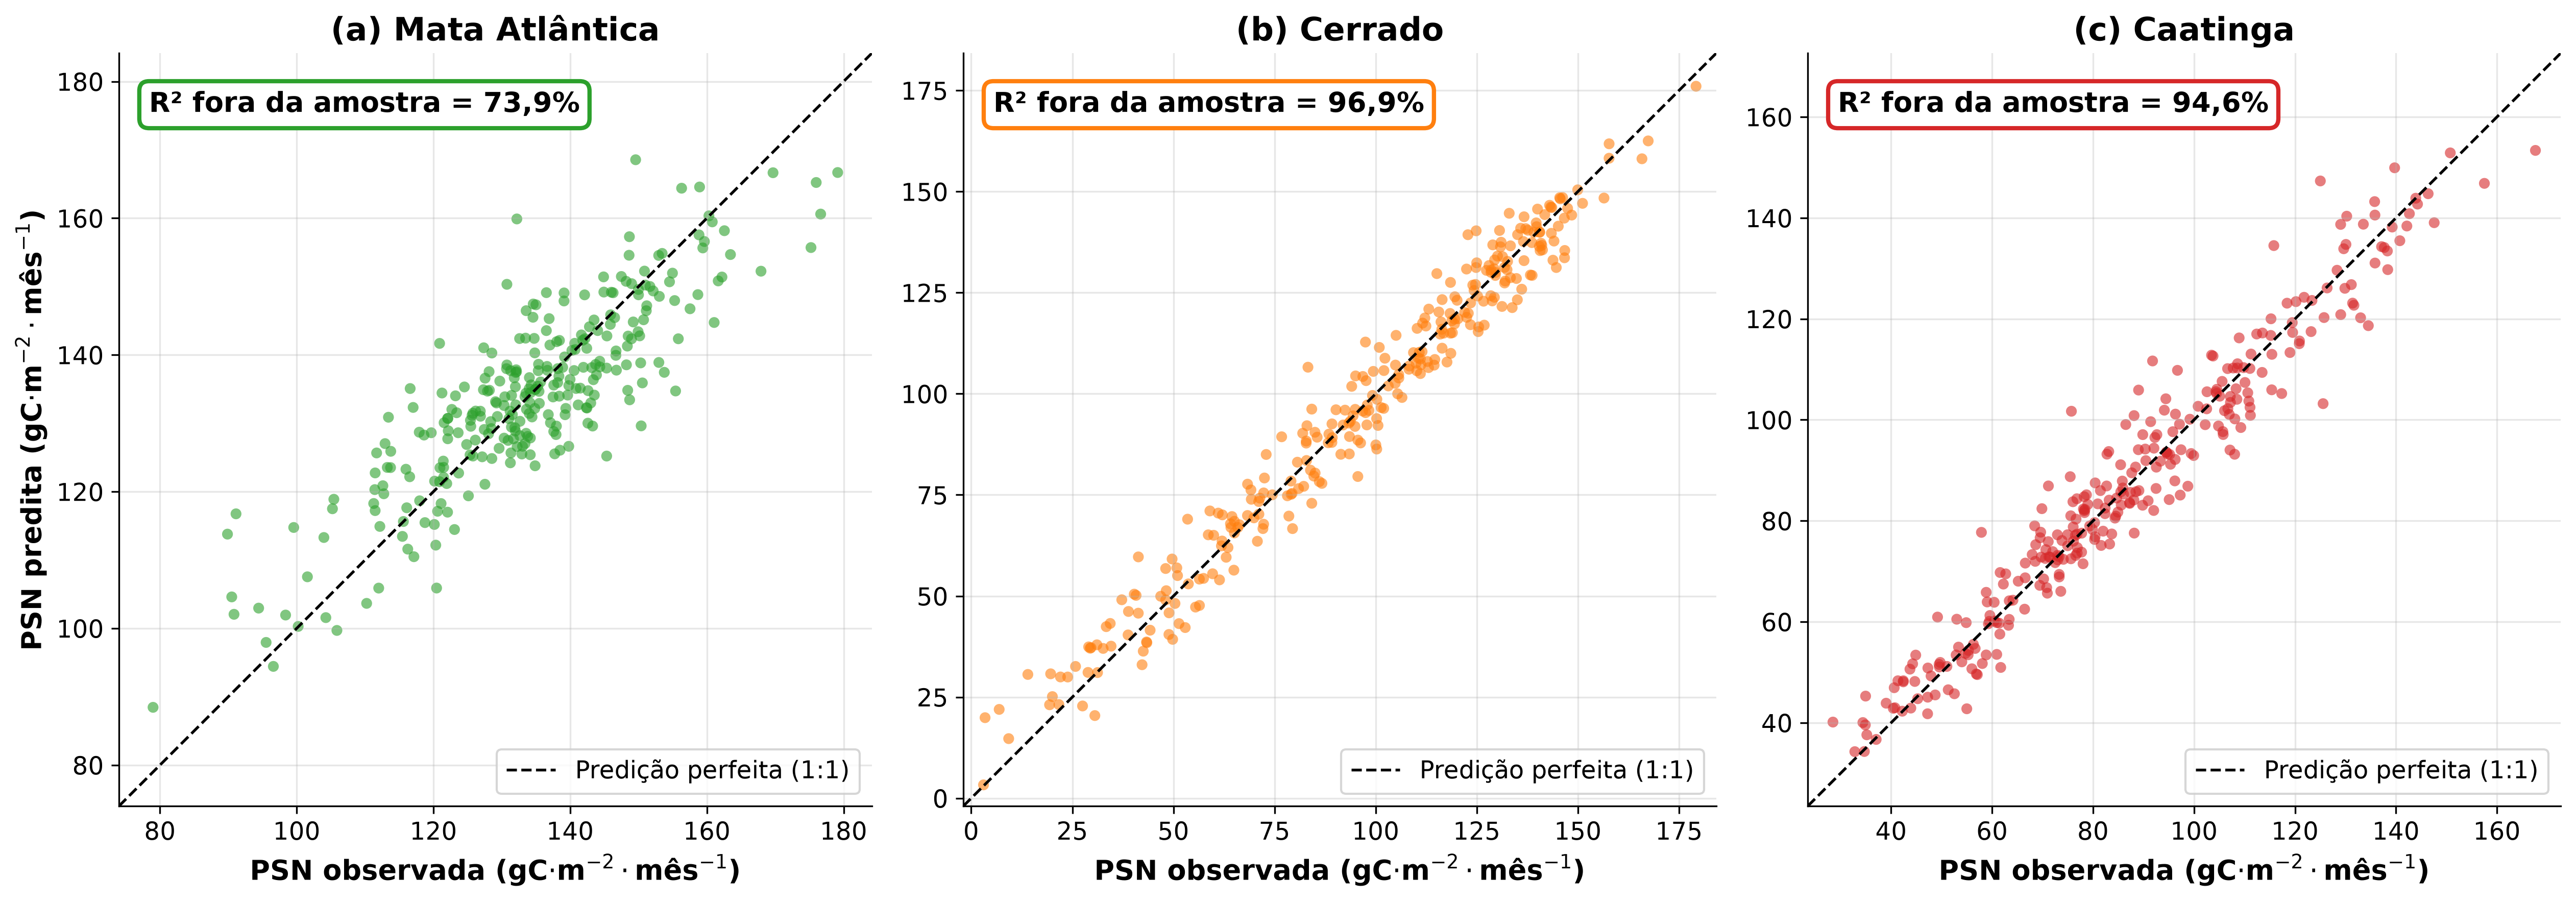
\includegraphics[width=\textwidth]{figs/fig3_obspred.png}
  \caption{PSN observada (MOD17A2HGF) e predita pelo MRMP-N nos três biomas, com predições fora da amostra obtidas por validação cruzada de cinco partições.}\label{fig:obspred}
\end{figure}

O grau 2 ofereceu o melhor compromisso entre desempenho de teste, estabilidade e parcimônia nos três biomas (Fig.~\ref{fig:degree}). O ganho em relação ao modelo linear foi de 8,4 pontos de $R^2$ de teste na Mata Atlântica (65,2\% para 73,6\%), 6,6 pontos no Cerrado (90,1\% para 96,7\%) e 1,3 ponto na Caatinga (92,9\% para 94,2\%). Na Mata Atlântica, o grau 3 alcançou $R^2$ 0,8 ponto superior ao do grau 2, com diferença treino--teste 1,7 ponto maior e 55 termos contra 20, e foi preterido pelo critério composto. Nos graus 4 e 5 o $R^2$ de teste caiu e a diferença treino--teste atingiu dezenas a centenas de pontos. A seleção do grau não dependeu do esquema de validação (Tabela~\ref{tbl:degtemp}). Refeita sob GroupKFold por ano e TimeSeriesSplit, a comparação indicou o grau 2 como o de maior $R^2$ de teste no Cerrado nos dois esquemas, e nos demais casos a vantagem de outro grau não passou de 0,8 ponto: grau 3 na Mata Atlântica sob GroupKFold (74,5\% contra 73,7\%) e grau 1 na Caatinga sob TimeSeriesSplit (91,5\% contra 91,2\%), ambos dentro da variação entre partições. Os graus 4 e 5 degradaram o desempenho em todos os esquemas.

\begin{table}[htbp]
\caption{$R^2$ de teste (\%) do MRMP-N por grau polinomial sob os três esquemas de validação, com o conjunto de variáveis selecionado de cada bioma.}\label{tbl:degtemp}
\footnotesize
\begin{tabular*}{\tblwidth}{@{}LCCCCC@{}}
\toprule
Bioma / esquema & Grau 1 & Grau 2 & Grau 3 & Grau 4 & Grau 5 \\
\midrule
Mata Atlântica, RepeatedKFold & 65,2 & 73,6 & 74,4 & 68,4 & 65,1 \\
Mata Atlântica, GroupKFold por ano & 65,5 & 73,7 & 74,5 & 67,4 & 67,2 \\
Mata Atlântica, TimeSeriesSplit & 58,7 & 67,0 & 61,0 & 56,3 & 53,9 \\
Cerrado, RepeatedKFold & 90,1 & 96,7 & 96,4 & 96,1 & 93,7 \\
Cerrado, GroupKFold por ano & 90,0 & 96,4 & 96,2 & 96,1 & 95,8 \\
Cerrado, TimeSeriesSplit & 88,5 & 95,7 & 93,7 & 93,4 & 92,2 \\
Caatinga, RepeatedKFold & 92,9 & 94,2 & 93,4 & 63,8 & 52,3 \\
Caatinga, GroupKFold por ano & 92,8 & 93,8 & 92,8 & 91,3 & 85,2 \\
Caatinga, TimeSeriesSplit & 91,5 & 91,2 & 90,4 & 87,0 & 86,7 \\
\bottomrule
\end{tabular*}
\end{table}

\begin{figure}
  \centering
  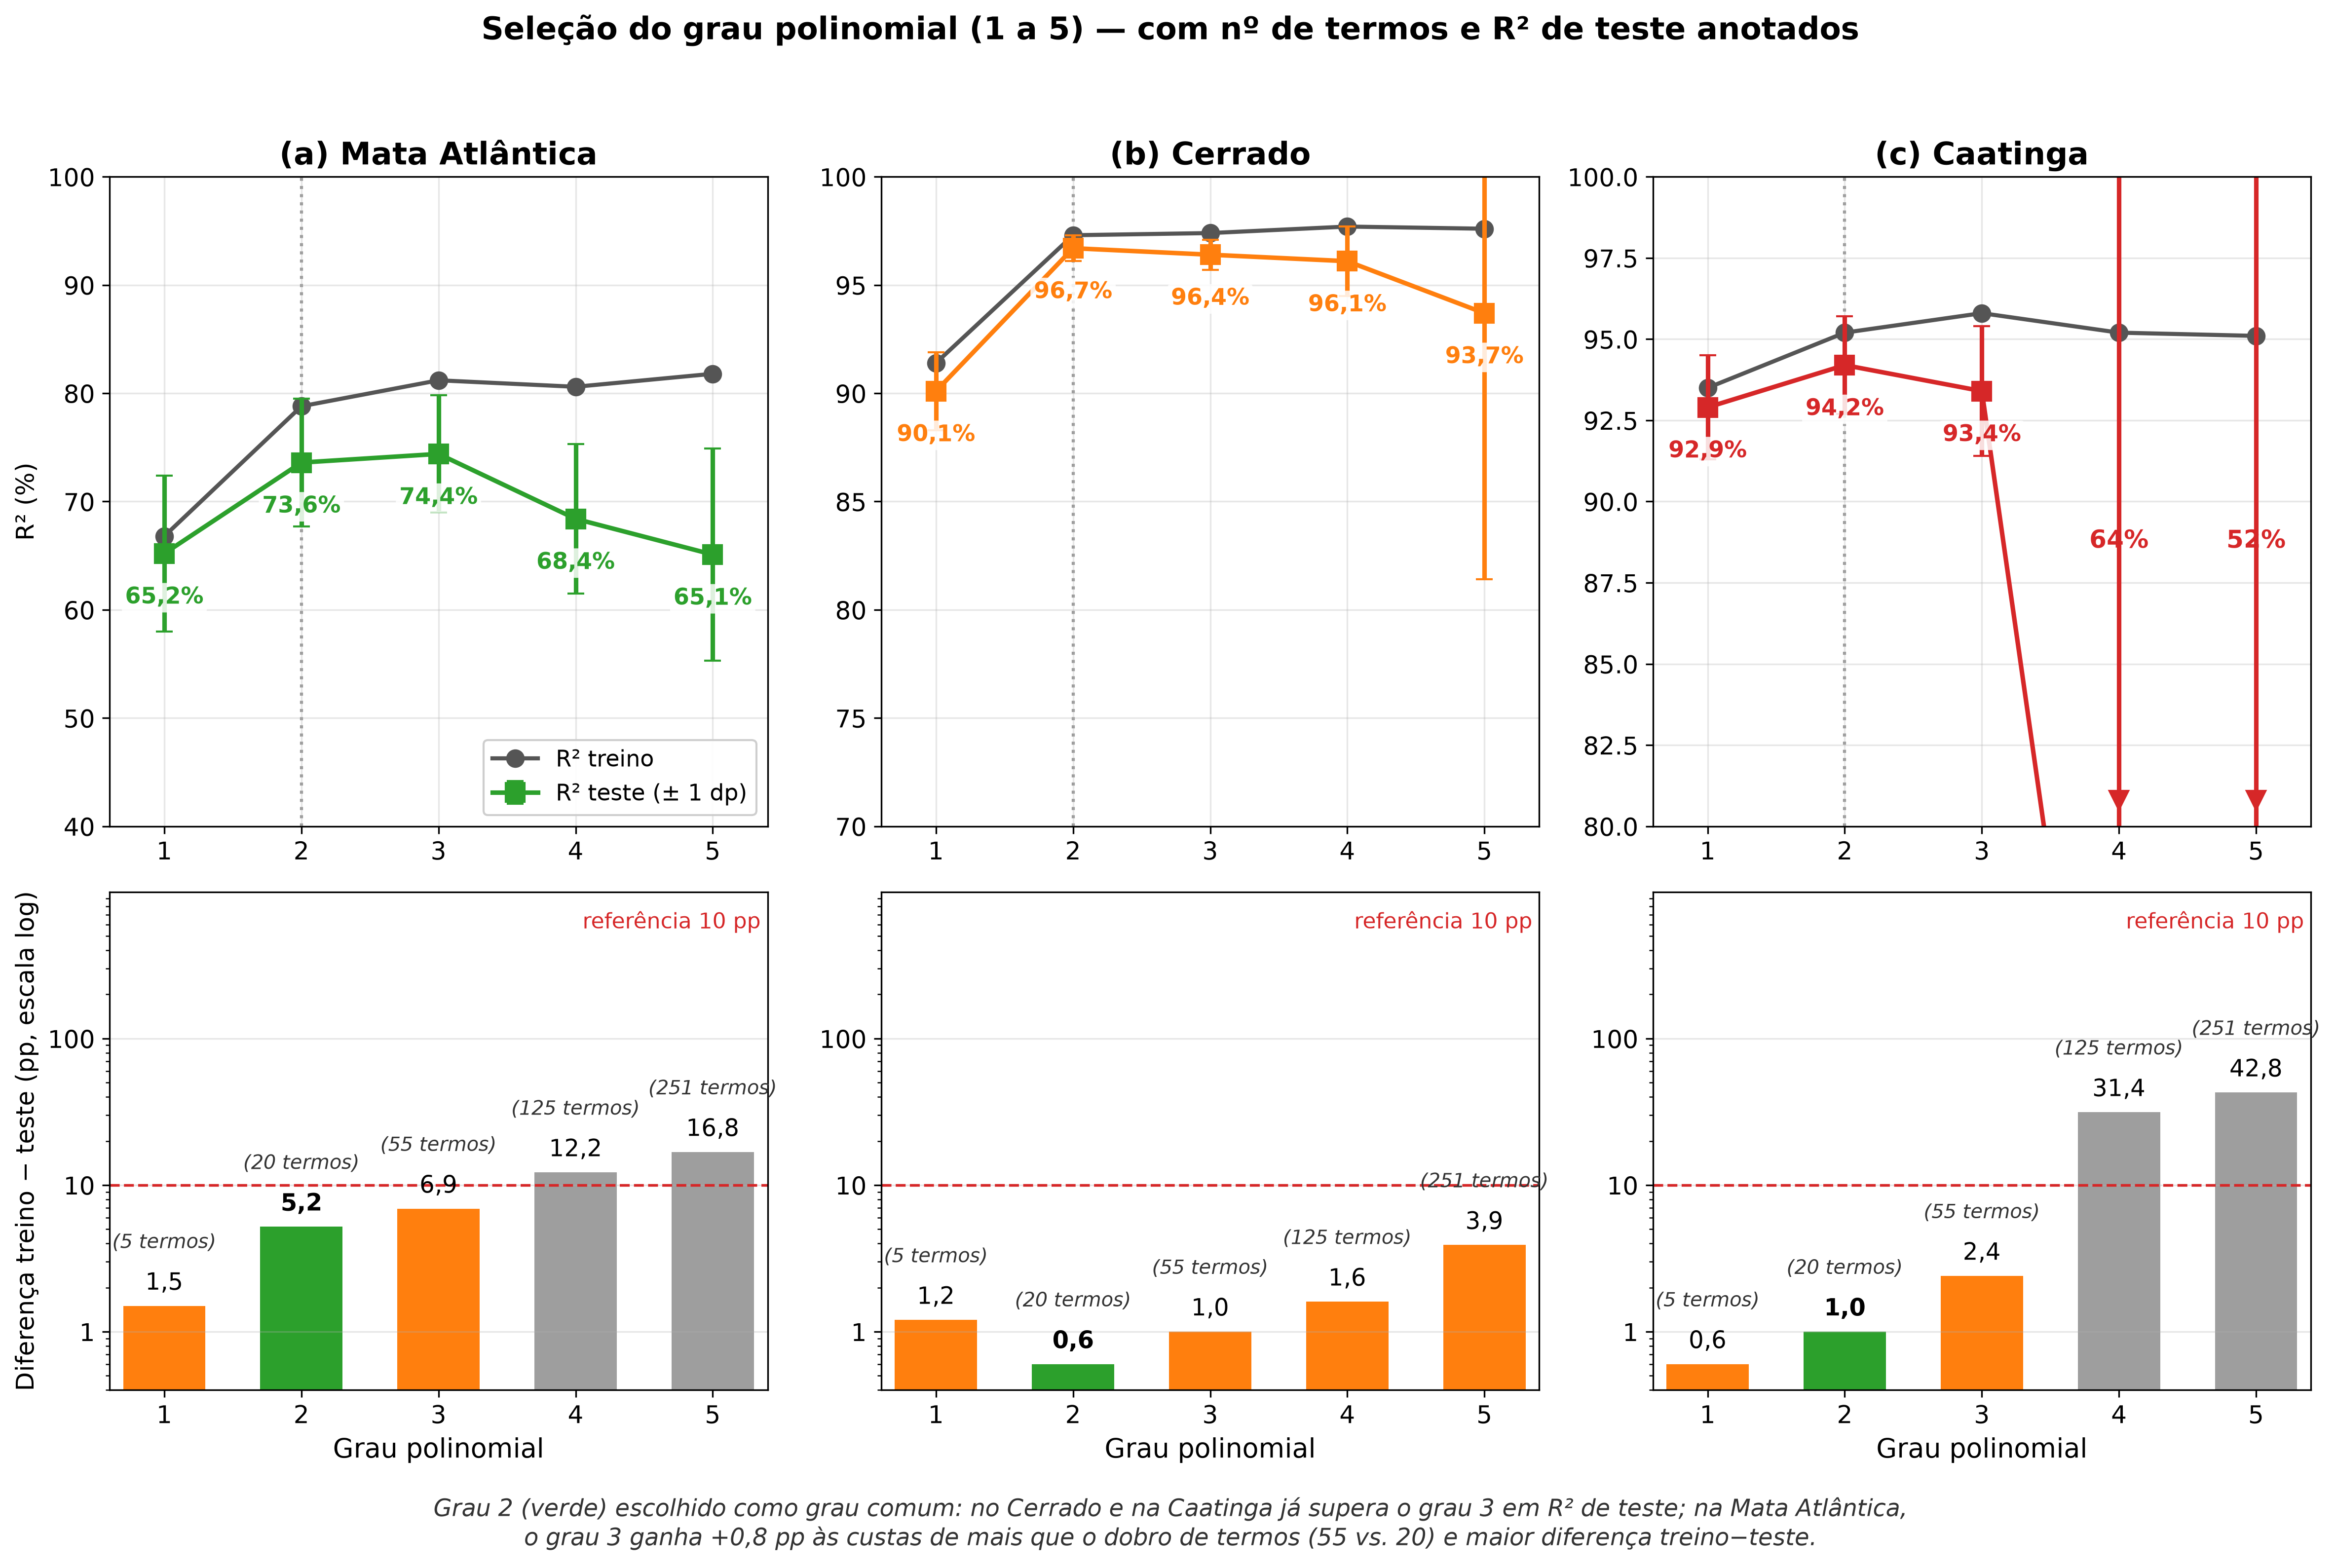
\includegraphics[width=\textwidth]{figs/fig4_degree.png}
  \caption{Seleção do grau polinomial do MRMP-N nos três biomas: $R^2$ de treino e de teste e diferença treino--teste por grau (RepeatedKFold $5 \times 30$).}\label{fig:degree}
\end{figure}

\subsection{Conjuntos de preditores e contribuição relativa}

Os conjuntos de preditores selecionados diferiram entre os biomas (Tabela~\ref{tbl:sets}). No Cerrado, o conjunto EV + PRE + WAI apresentou a menor diferença treino--teste de todas as combinações e foi o melhor em 83\% das 150 partições; sua diferença pareada de $R^2$ de teste em relação a EV + PRE + TST foi de 0,39 ponto (IC 95\% por bootstrap: 0,33 a 0,45; Wilcoxon, $p < 0,001$), positiva em 86\% das partições, e o conjunto ocupou o primeiro lugar também sob GroupKFold por ano e TimeSeriesSplit. Na Mata Atlântica, EV + TST + WAI foi o melhor em 66\% das partições e em primeiro nos dois esquemas temporais. Na Caatinga, as três melhores combinações ficaram separadas por menos de 0,3 ponto: EV + PRE + TST foi o melhor em 36\% das partições e ficou em primeiro sob GroupKFold e em segundo sob TimeSeriesSplit, atrás de EV + PRE + WAI (91,9\% contra 91,2\%), sendo a escolha menos estável dos três biomas. Na Mata Atlântica, o conjunto EV + TST + WAI superou em 2,7 pontos a combinação EV + PRE + TST, embora o WAI, isoladamente, explique menos de 2\% da variância da PSN nesse bioma. A área queimada não integrou o conjunto selecionado de nenhum bioma. A evapotranspiração apresentou o maior índice de contribuição relativa nos três biomas (26,9\% na Mata Atlântica, 37,4\% no Cerrado e 42,8\% na Caatinga), e as componentes harmônicas somaram entre 32\% e 40\% do índice em cada bioma (Fig.~\ref{fig:contrib}).

\begin{table}[htbp]
\caption{Três melhores combinações de variáveis ambientais por bioma (mais SAZsin e SAZcos), grau 2: $R^2$ de treino e de teste e diferença treino--teste sob RepeatedKFold $5 \times 30$, frequência com que a combinação foi a melhor entre as 150 partições, e posição sob GroupKFold por ano e TimeSeriesSplit.}\label{tbl:sets}
\footnotesize
\begin{tabular*}{\tblwidth}{@{}LLCCCCCC@{}}
\toprule
Bioma & Variáveis & $R^2$ treino (\%) & $R^2$ teste (\%) & Dif.\ (pp) & Melhor em (\%) & Posição por ano & Posição cronológica \\
\midrule
Mata Atlântica & EV + TST + WAI & 78,8 & 73,6 & 5,2 & 66,0 & 1º & 1º \\
 & EV + PRE + TST & 76,1 & 71,0 & 5,1 & 19,3 & 2º & 2º \\
 & EV + PRE + WAI & 74,4 & 69,0 & 5,4 & 12,0 & 3º & 3º \\
Cerrado & EV + PRE + WAI & 97,3 & 96,7 & 0,6 & 82,7 & 1º & 1º \\
 & EV + PRE + TST & 97,0 & 96,3 & 0,7 & 14,0 & 2º & 2º \\
 & EV + PRE + BURN & 96,9 & 95,8 & 1,2 & 2,7 & 3º & 3º \\
Caatinga & EV + PRE + TST & 95,2 & 94,2 & 1,0 & 36,0 & 1º & 2º \\
 & EV + PRE + WAI & 95,1 & 94,0 & 1,1 & 22,0 & 2º & 1º \\
 & PRE + TST + WAI & 95,0 & 93,9 & 1,1 & 28,7 & 4º & 5º \\
\bottomrule
\end{tabular*}
\end{table}

\begin{figure}
  \centering
  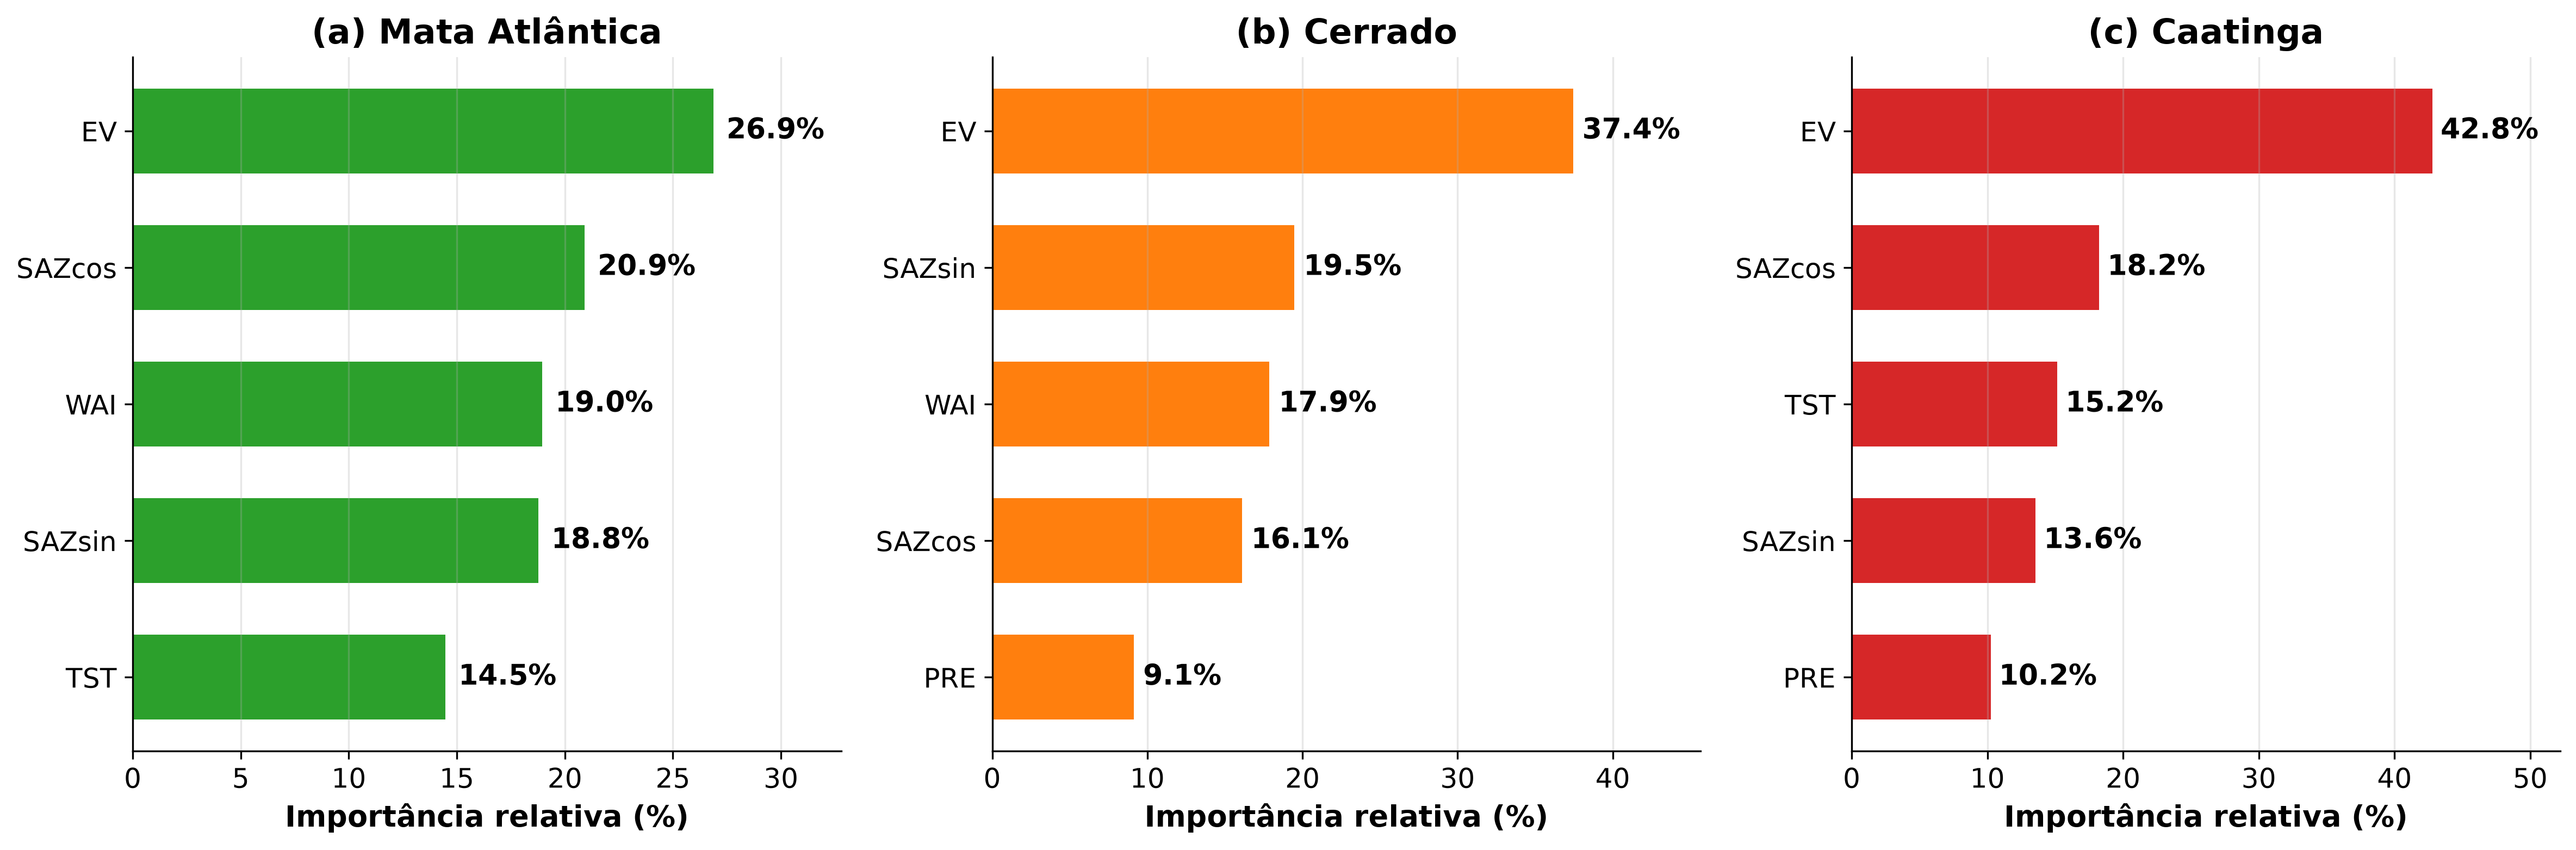
\includegraphics[width=\textwidth]{figs/fig5_contribution.png}
  \caption{Índice de contribuição relativa das variáveis preditoras no MRMP-N de grau 2 nos três biomas.}\label{fig:contrib}
\end{figure}

A importância por permutação fora da amostra (Tabela~\ref{tbl:perm}) coincidiu com o índice de coeficientes no preditor dominante, a evapotranspiração, mas lhe atribuiu parcela muito maior: 42\% da queda total do $R^2$ na Mata Atlântica, 85\% no Cerrado e 80\% na Caatinga sob GroupKFold por ano, com parcelas semelhantes sob TimeSeriesSplit. As duas medidas divergiram nas variáveis secundárias: no Cerrado, o WAI recebeu 3\% da queda total sob permutação, contra 18\% do índice de coeficientes, porque grande parte de sua informação é partilhada com a EV. Os valores absolutos das quedas são grandes porque o embaralhamento de um preditor central leva os termos quadráticos e de interação a extrapolar.

\begin{table}[htbp]
\caption{Importância por permutação fora da amostra: parcela de cada variável na queda total do $R^2$ de teste (\%, média $\pm$ desvio-padrão entre os cinco blocos, 20 embaralhamentos por bloco) e razão entre o RMSE com e sem embaralhamento, sob GroupKFold por ano e TimeSeriesSplit.}\label{tbl:perm}
\footnotesize
\begin{tabular*}{\tblwidth}{@{}LLCCCC@{}}
\toprule
Bioma & Variável & Parcela por ano (\%) & Razão RMSE por ano & Parcela cronológica (\%) & Razão RMSE cronológica \\
\midrule
Mata Atlântica & EV & 41,9 $\pm$ 7,7 & 4,16 & 38,2 $\pm$ 6,4 & 3,47 \\
 & WAI & 21,1 $\pm$ 5,0 & 3,01 & 19,9 $\pm$ 5,1 & 2,64 \\
 & SAZcos & 16,6 $\pm$ 2,5 & 2,74 & 16,7 $\pm$ 2,7 & 2,43 \\
 & SAZsin & 11,0 $\pm$ 1,2 & 2,29 & 15,2 $\pm$ 3,8 & 2,34 \\
 & TST & 9,4 $\pm$ 3,8 & 2,10 & 10,0 $\pm$ 4,5 & 1,89 \\
Cerrado & EV & 85,3 $\pm$ 1,4 & 11,25 & 77,7 $\pm$ 15,1 & 10,24 \\
 & SAZcos & 4,4 $\pm$ 0,6 & 2,74 & 6,1 $\pm$ 3,6 & 2,70 \\
 & PRE & 4,1 $\pm$ 0,8 & 2,62 & 3,7 $\pm$ 0,4 & 2,41 \\
 & SAZsin & 3,6 $\pm$ 0,6 & 2,50 & 5,0 $\pm$ 1,9 & 2,59 \\
 & WAI & 2,6 $\pm$ 0,9 & 2,15 & 7,5 $\pm$ 10,2 & 2,46 \\
Caatinga & EV & 80,4 $\pm$ 2,5 & 6,81 & 76,9 $\pm$ 10,0 & 5,13 \\
 & SAZcos & 8,9 $\pm$ 1,5 & 2,48 & 4,7 $\pm$ 2,3 & 1,65 \\
 & SAZsin & 4,6 $\pm$ 1,0 & 1,90 & 3,2 $\pm$ 1,5 & 1,47 \\
 & TST & 3,7 $\pm$ 1,2 & 1,75 & 11,4 $\pm$ 13,4 & 1,82 \\
 & PRE & 2,4 $\pm$ 1,2 & 1,48 & 3,8 $\pm$ 2,3 & 1,42 \\
\bottomrule
\end{tabular*}
\end{table}

\subsection{Papel das componentes harmônicas}

A remoção das componentes harmônicas reduziu o $R^2$ de teste em 21,8 pontos na Mata Atlântica, 3,0 pontos no Cerrado e 2,4 pontos na Caatinga (Tabela~\ref{tbl:harm}). No Cerrado, entre 70\% e 79\% da variância da evapotranspiração e do WAI foi explicada pelo ciclo anual, contra cerca de 40\% na Mata Atlântica. Na presença dos harmônicos, a contribuição da precipitação caiu de 29,0\% para 9,1\% no Cerrado e de 24,1\% para 10,2\% na Caatinga, e a da temperatura caiu de 40,3\% para 14,5\% na Mata Atlântica, enquanto a da evapotranspiração se manteve ou aumentou. A correlação entre as anomalias mensais da evapotranspiração e da PSN variou de 0,73 a 0,93, enquanto a da precipitação foi de 0,02 no Cerrado e 0,16 na Caatinga.

\begin{table}[htbp]
\caption{Efeito das componentes harmônicas: $R^2$ de teste do MRMP-N com e sem sazonalidade explícita, proporção da variância de cada preditor explicada pelo ciclo anual, correlação das anomalias mensais com a PSN e índice de contribuição relativa sem e com harmônicos. Os harmônicos receberam entre 32\% e 40\% do índice total em cada bioma. Anomalia = desvio em relação à média do mês do calendário na série.}\label{tbl:harm}
\scriptsize
\begin{tabular*}{\tblwidth}{@{}LCLCCCC@{}}
\toprule
Bioma & $R^2$ com / sem (\%) & Variável & $R^2$ ciclo anual (\%) & $r$ anomalias & Índice sem (\%) & Índice com (\%) \\
\midrule
Mata Atlântica & 73,7 / 51,9 & EV & 39,8 & 0,73 & 27,0 & 26,9 \\
 & & TST & 64,9 & $-$0,58 & 40,3 & 14,5 \\
 & & WAI & 39,8 & 0,42 & 32,8 & 19,0 \\
Cerrado & 96,7 / 93,7 & EV & 79,1 & 0,90 & 34,7 & 37,4 \\
 & & PRE & 58,9 & 0,02 & 29,0 & 9,1 \\
 & & WAI & 70,2 & 0,76 & 36,2 & 17,9 \\
Caatinga & 94,2 / 91,8 & EV & 63,3 & 0,93 & 49,5 & 42,8 \\
 & & PRE & 31,5 & 0,16 & 24,1 & 10,2 \\
 & & TST & 54,2 & $-$0,77 & 26,4 & 15,2 \\
\bottomrule
\end{tabular*}
\end{table}

\subsection{Diagnóstico, Y-randomization e nulos temporais}

O VIF ficou abaixo de 5,1 para todos os preditores na Mata Atlântica e na Caatinga; no Cerrado, a evapotranspiração e o WAI apresentaram VIF de 36,99 e 31,61. Os resíduos foram normais na Mata Atlântica (Shapiro--Wilk, $p = 0,630$) e no Cerrado ($p = 0,423$) e apresentaram desvio na cauda esquerda na Caatinga ($p = 0,002$). O teste de Ljung--Box detectou autocorrelação residual nos três biomas ($p \le 0,005$), com autocorrelação de defasagem 1 de 0,51 na Mata Atlântica, 0,20 no Cerrado e 0,42 na Caatinga. No teste de Y-randomization, os modelos ajustados à PSN permutada tiveram $R^2$ de validação cruzada médio de $-10,6\%$, $-10,9\%$ e $-13,0\%$, contra 73,8\%, 96,7\% e 94,2\% dos modelos originais, distâncias de 84,4, 107,5 e 107,2 pontos; nenhuma das 100 permutações igualou o modelo original ($p = 0,0099$). Sob os nulos que preservam a estrutura temporal (Tabela~\ref{tbl:nulls}), os modelos nulos alcançaram $R^2$ médio bem superior ao da permutação livre, sobretudo com a permutação de anos inteiros (62,4\% no Cerrado e 40,2\% na Caatinga), que mantém a sazonalidade e a memória da série, mas nenhum nulo alcançou o modelo original em nenhum bioma ($p$ empírico entre 0,003 e 0,040).

\begin{table}[htbp]
\caption{Nulos que preservam a estrutura temporal da PSN: $R^2$ de validação cruzada (RepeatedKFold $5 \times 30$, $\alpha$ fixo) do modelo original e dos modelos nulos por deslocamento circular da PSN (todos os 296 deslocamentos e o subconjunto dos múltiplos de 12 meses) e por permutação de anos inteiros (100 permutações). $p$ empírico = (nº de nulos com $R^2 \ge$ original + 1)/($n$ + 1).}\label{tbl:nulls}
\footnotesize
\begin{tabular*}{\tblwidth}{@{}LLCCCCC@{}}
\toprule
Bioma & Nulo & $n$ & $R^2$ original (\%) & $R^2$ nulo, média $\pm$ dp (\%) & $R^2$ nulo, máx.\ (\%) & $p$ empírico \\
\midrule
Mata Atlântica & Deslocamento circular & 296 & 73,8 & $-$3,0 $\pm$ 6,1 & 52,4 & 0,003 \\
 & Deslocamento múltiplo de 12 meses & 24 & 73,8 & $-$3,2 $\pm$ 5,0 & 7,3 & 0,040 \\
 & Permutação de anos & 100 & 73,8 & 4,4 $\pm$ 2,7 & 11,5 & 0,010 \\
Cerrado & Deslocamento circular & 296 & 96,7 & 36,3 $\pm$ 12,9 & 81,8 & 0,003 \\
 & Deslocamento múltiplo de 12 meses & 24 & 96,7 & 35,5 $\pm$ 11,0 & 58,7 & 0,040 \\
 & Permutação de anos & 100 & 96,7 & 62,4 $\pm$ 1,4 & 67,0 & 0,010 \\
Caatinga & Deslocamento circular & 296 & 94,2 & 23,9 $\pm$ 8,9 & 72,5 & 0,003 \\
 & Deslocamento múltiplo de 12 meses & 24 & 94,2 & 22,5 $\pm$ 7,4 & 36,5 & 0,040 \\
 & Permutação de anos & 100 & 94,2 & 40,2 $\pm$ 2,3 & 44,7 & 0,010 \\
\bottomrule
\end{tabular*}
\end{table}

\section{Discussão}\label{sec:discussion}

\subsection{Associações climáticas da fotossíntese líquida nos biomas}

Os três biomas configuram um gradiente de previsibilidade climática da PSN. O elevado desempenho no Cerrado reflete a forte sazonalidade hídrica do bioma, na qual a alternância entre estações seca e chuvosa impõe um ritmo regular à atividade fotossintética; estudos com torres de fluxo mostram que a produtividade primária do Cerrado acompanha o conteúdo de água no solo e a precipitação \citep{arruda2016,biudes2021,vourlitis2022}. Na Caatinga, a previsibilidade decorre do regime de pulsos de recursos característico de ambientes semiáridos, em que a vegetação responde de forma quase imediata aos eventos de chuva \citep{schwinning2004,mendes2025,silva2026}, o que é coerente com o ganho marginal do grau 2 sobre o modelo linear nesse bioma. O desempenho inferior na Mata Atlântica reflete a diversidade de tipos climáticos da faixa litorânea \citep{alvares2013} e a heterogeneidade estrutural do bioma mais fragmentado do estado, no qual o histórico de desmatamento, a silvicultura de eucalipto e o efeito de borda introduzem fontes de variabilidade não capturáveis por preditores climáticos regionais \citep{lima2020,broggio2024}. \citet{benfica2023} já haviam observado, nas mesmas séries, correlações mais fortes entre a PSN e as variáveis hídricas no Cerrado e na Caatinga e menor variação sazonal na Mata Atlântica; os resultados aqui obtidos quantificam essa diferença como um gradiente de previsibilidade e a organizam em três padrões de associação: limitação hídrica sazonal no Cerrado, resposta pulsada à chuva na Caatinga e resposta multifatorial na Mata Atlântica.

O resultado mais relevante da seleção de variáveis foi a escolha do WAI em lugar da TST na combinação de melhor desempenho do Cerrado. A preferência é estatisticamente consistente, com diferença pareada positiva em 86\% das partições e primeiro lugar nos três esquemas de validação, mas de magnitude pequena, 0,4 ponto de $R^2$; o resultado indica, portanto, redundância da temperatura na presença do WAI, e não sua irrelevância ecológica. Além disso, como EV e WAI compartilham grande parte da informação nesse bioma (VIF acima de 30) e o WAI recebe apenas 3\% da importância por permutação, suas contribuições individuais devem ser lidas com cautela. No Cerrado, a temperatura atua primariamente sobre o balanço hídrico, elevando a demanda evaporativa e reduzindo a disponibilidade de água no solo, processo determinante para a fisiologia da vegetação savânica \citep{bucci2008,arruda2016}. O WAI, definido como a razão entre a evapotranspiração real e a potencial, expressa o grau em que a demanda atmosférica por água é atendida pela água disponível no sistema e integra, em uma única variável, os efeitos combinados da temperatura e da precipitação. A literatura sobre savanas tropicais aponta a limitação hídrica sazonal, e não a térmica, como principal controle da produtividade \citep{vourlitis2022}. Sob as projeções de intensificação das secas e de aumento da demanda evapotranspirativa para o Brasil Central \citep{ipcc2022}, e considerando que a produtividade responde de forma não linear à disponibilidade hídrica \citep{mwangi2025}, o WAI constitui um indicador quantitativo de vulnerabilidade climática do Cerrado baiano, passível de uso no monitoramento de tendências de produtividade.

Uma ressalva sobre a origem dos dados aplica-se à associação entre a PSN e a evapotranspiração. A PSN (MOD17A2HGF) e a EV (MOD16A2GF) são estimadas por algoritmos da mesma família, que partilham entradas: ambos utilizam a fração da radiação fotossinteticamente ativa absorvida e o índice de área foliar do produto MOD15A2H, a classificação de cobertura do solo do MCD12Q1 e os mesmos campos meteorológicos de reanálise do GMAO/MERRA-2 \citep{running2004,running2021gpp,running2021et}. Parte da forte associação entre EV e PSN observada nos três biomas pode, portanto, refletir dependência algorítmica entre os produtos, e não apenas o acoplamento ecofisiológico entre transpiração e assimilação de carbono pelos estômatos \citep{lawson2019}. Essa dependência não invalida o uso do modelo para o fim proposto, que é representar e prever a PSN estimada pelo MOD17 a partir de variáveis disponíveis na mesma escala; e a associação da PSN com a precipitação (IMERG) e com a temperatura da superfície (MOD11A2), produtos independentes do MOD17, aponta na mesma direção, assim como a variação da associação univariada de 12,5\% na Mata Atlântica a 76\% na Caatinga, que não ocorreria se o algoritmo compartilhado fosse o fator dominante. Ela recomenda, contudo, cautela ao interpretar a magnitude da contribuição da EV como evidência ecológica autônoma. A validação das relações com dados independentes, como as medições de fluxo por covariância de vórtices disponíveis para a Caatinga \citep{mendes2020,mendes2025} e para o Cerrado \citep{vourlitis2022}, é indicada como etapa futura.

Na Mata Atlântica, o WAI integrou o conjunto selecionado e recebeu 19\% do índice de contribuição apesar de explicar menos de 2\% da PSN isoladamente. Essa contribuição surge exclusivamente por interação com a evapotranspiração e a temperatura: em um bioma úmido, não limitado por água em condições médias, a disponibilidade hídrica importa apenas quando combinada a condições térmicas ou de demanda evaporativa específicas. Um modelo aditivo não capturaria esse efeito, o que explica por que o grau 2 ganhou mais sobre o linear justamente nesse bioma. A ausência da área queimada no conjunto selecionado de qualquer bioma indica que, na escala mensal e espacial adotada, essa variável não acrescentou poder preditivo suficiente em relação aos demais preditores. Isso não implica ausência de efeito ecológico do fogo, documentado na Bahia por \citet{benfica2022,benfica2023} e em savanas tropicais por \citet{navarro2025}, e pode refletir a heterogeneidade espacial das queimadas dentro de cada bioma, respostas defasadas da produtividade e informação compartilhada com os preditores hídricos.

\subsection{Sazonalidade explícita, regularização e validação}

A análise com e sem componentes harmônicas oferece uma contribuição que transcende o caso estudado. Em séries mensais de produtividade, grande parte da variância é determinística: fotoperíodo, radiação e fenologia foliar impõem um ciclo anual que qualquer variável climática sazonal reproduz parcialmente \citep{wu2016,alberton2019}. Quando o ciclo não é representado explicitamente, a precipitação e a temperatura recebem crédito pelo calendário e sua contribuição é superestimada. Quando os harmônicos absorvem o ciclo, cada preditor é avaliado pela informação que acrescenta além do ano típico, isto é, pelas anomalias. Os resultados mostram que a chuva do próprio mês é um fluxo de entrada ruidoso e defasado, com correlação quase nula com a anomalia de PSN no Cerrado, enquanto a evapotranspiração mede a água efetivamente utilizada pela vegetação e acompanha de perto a anomalia de produtividade, porque transpiração e assimilação de carbono ocorrem pelos mesmos estômatos \citep{lawson2019}. A acentuada perda de desempenho ao remover a sazonalidade na Mata Atlântica sugere que a PSN desse bioma responde a um componente do ciclo anual, possivelmente fotoperíodo ou fenologia foliar \citep{borchert2001,wu2016}, não inteiramente representado pelas variáveis climáticas medidas. Recomenda-se, portanto, que estudos de contribuição de variáveis em séries mensais de produtividade incluam termos de sazonalidade explícitos.

A escolha do grau 2 nos três biomas deve ser lida de forma restrita: dentro do conjunto de variáveis e do intervalo de graus avaliados, os termos quadráticos e de interação entre pares foram suficientes para obter o melhor compromisso entre desempenho de teste e complexidade do modelo, e graus superiores não acrescentaram estrutura preditiva que compensasse o aumento do número de termos e do sobreajuste. A regularização foi decisiva: no Cerrado, os VIF de 37 e 32 para a evapotranspiração e o WAI tornariam a estimação por mínimos quadrados instável, enquanto a penalização L2 manteve o modelo estável sob todas as estratégias de validação. A concordância entre a validação cruzada repetida e os esquemas cronológicos indica que o desempenho não decorre de meses vizinhos terem caído simultaneamente no treino e no teste, e a manutenção do grau 2 e dos conjuntos selecionados quando a própria seleção é feita sob os esquemas temporais afasta a objeção de que a escolha dos hiperparâmetros dependeria do embaralhamento dos meses. O contraste entre o índice de coeficientes e a importância por permutação reforça a leitura do primeiro como descrição da estrutura do modelo ajustado, e não como medida de importância no sentido estrito: o índice reparte o peso entre termos correlacionados, ao passo que a permutação atribui a cada variável apenas a informação que ela carrega além das demais. Os nulos que preservam a estrutura temporal mostram que a sazonalidade e a memória da série explicam, por si sós, parcela substancial do $R^2$ nos biomas sazonais, mas a diferença entre o modelo original e esses nulos quantifica o ganho que decorre do alinhamento entre a PSN e as condições climáticas do próprio período, maior nos biomas sazonais e menor na Mata Atlântica. A autocorrelação residual detectada nos três biomas indica memória temporal não modelada, como a água armazenada no solo \citep{oliveira2005}, e não impediu que a capacidade preditiva permanecesse elevada sob validação cronológica; a incorporação de preditores defasados ou termos autorregressivos é a extensão natural do modelo. Outras limitações devem ser reconhecidas: a modelagem não incorporou variáveis estruturais da paisagem, potencialmente relevantes para a variabilidade residual da Mata Atlântica; a escala mensal limita a representação de eventos extremos de curta duração; a abordagem é correlacional e não permite inferências causais; e o modelo estima a PSN de um mês a partir das variáveis desse mesmo mês, não gerando previsões autônomas do futuro. A seleção do conjunto de variáveis foi feita sobre as mesmas partições usadas para reportar o desempenho, e não em esquema totalmente aninhado, o que pode introduzir algum otimismo de seleção, atenuado pelas validações agrupada por ano e cronológica. Três limitações de origem dos dados devem ainda ser explicitadas: a PSN e a EV provêm de algoritmos MODIS que compartilham entradas; a temperatura da superfície não passou por filtro pela banda de qualidade QC\_Day, e a sensibilidade da série a esse filtro não foi avaliada; e os períodos aqui chamados mensais são janelas fixas de 32 dias associadas a um mês civil de referência. A comparação com modelos aditivos generalizados e florestas aleatórias sob o mesmo protocolo permitiria situar o custo, se houver, da interpretabilidade que a estrutura polinomial oferece.

\section{Conclusões}\label{sec:conclusions}

O modelo de regressão múltipla polinomial de grau 2, estimado por regressão Ridge, explicou 96,7\%, 94,2\% e 73,7\% da variância mensal da PSN no Cerrado, na Caatinga e na Mata Atlântica da Bahia entre 2001 e 2025, com desempenho estável sob validação cruzada repetida, validação cronológica e Y-randomization. A seleção do grau e dos conjuntos manteve-se quando refeita sob validação agrupada por ano e cronológica, e o desempenho superou nulos que preservam a sazonalidade e a autocorrelação da série. Os conjuntos de preditores selecionados diferiram entre os biomas: o índice de disponibilidade hídrica foi selecionado em lugar da temperatura no Cerrado, onde integra a informação térmica e hídrica, e contribuiu por interação na Mata Atlântica. A representação explícita do ciclo anual mostrou-se essencial no bioma úmido e alterou a interpretação da contribuição das variáveis, que passa a refletir anomalias e não o calendário. Os três biomas apresentam padrões distintos de associação entre clima e produtividade, o que reforça a necessidade de estratégias de monitoramento diferenciadas por bioma: em biomas limitados pela água, um conjunto reduzido de variáveis de sensoriamento remoto é suficiente para acompanhar a PSN; na Mata Atlântica, recomenda-se a incorporação de variáveis estruturais da paisagem em estudos futuros. A regressão polinomial regularizada com seleção empírica de grau e de variáveis e validação temporal constitui uma alternativa reprodutível e interpretável para representar relações ambientais não lineares com dados orbitais, aplicável a outras regiões com gradientes ambientais semelhantes.

\section*{Disponibilidade de dados}
A base mensal (297 períodos por bioma, 2001--2025), o código em Python do modelo e de todas as validações e os resultados da rodada completa estão disponíveis em \url{https://github.com/heroslore/MRMP-N-PSN-Bahia} e arquivados de forma permanente no Zenodo sob o DOI \url{https://doi.org/10.5281/zenodo.22883915} (versão utilizada neste trabalho: v1.0.0, \url{https://doi.org/10.5281/zenodo.22883916}). A base é também fornecida como material suplementar (arquivo CSV).

\section*{Declaração de conflito de interesses}
Os autores declaram não haver conflitos de interesse financeiros ou pessoais que pudessem ter influenciado o trabalho relatado neste artigo.

\section*{Agradecimentos}
O presente trabalho foi realizado com apoio da Coordenação de Aperfeiçoamento de Pessoal de Nível Superior -- Brasil (CAPES) -- Código de Financiamento 001, por meio de bolsa de mestrado concedida ao primeiro autor. Os autores agradecem ao Programa de Pós-graduação em Ciências e Tecnologias Ambientais (UFSB/IFBA). O primeiro autor agradece ao Prof. Dr. Fabrício Berton Zanchi, pela orientação, e à Profa. Dra. Nayanne Silva Benfica, pela coorientação.

\printcredits

\bibliographystyle{cas-model2-names}
\bibliography{refs}

\end{document}
